\documentclass[10pt]{article}
\usepackage{natbib}
\usepackage[fontset=windows]{ctex}
\usepackage{amsmath}
\usepackage{amssymb}
\usepackage{color}
\usepackage{colortbl}
\usepackage{verbatim}		%Add comments
\usepackage{listings}		%Add codes
\usepackage{xcolor}			%代码高亮

\usepackage{multirow}
\usepackage{longtable}
\usepackage{array}
\usepackage{makecell}
\usepackage{threeparttable}
\usepackage{siunitx}
\usepackage{booktabs}

\renewcommand{\baselinestretch}{1.25}

\usepackage{graphicx}
\usepackage{float}
\usepackage{subfigure}
\usepackage{caption}

\usepackage{setspace}
\usepackage{geometry}
\geometry{left=3.17cm,right=3.17cm,top=2.54cm,bottom=2.54cm}

\begin{document}

\title{\fontsize{36pt}{36pt}\selectfont% 
	{\songti% 黑体 
        四足机器狗总体设计和\protect\\
		建模仿真}}

\author{\fontsize{12pt}{18pt}\selectfont% 小四字号，1.5倍行距
	{\fangsong% 仿宋
		侯红日PB19050979}\\
	\fontsize{10.5pt}{15.75pt}\selectfont% 五号字号，1.5倍行距
	{\fangsong% 仿宋
		(中国科学技术大学~~~精密机械与精密仪器系)}}% 作者单位，“~”表示空格
\date{\today}

\maketitle

\pagenumbering{roman}
\pagenumbering{arabic}

\begin{abstract}
	机器人诞生的初衷在于服务人类，将人类从重复、繁琐甚至危险的工作中解放出来，进而把有限的人力资源投入到更有价值的生产劳动过程中去。波士顿动力公司成立于 1992 年，主要开展机器人相关研究工作，其目标是打造像人或动物那样，能够在现实世界中灵活工作的智能机器人。而本文则主要尝试复现波士顿动力公司的四足机器狗，通过Solidworks软件对机器狗进行建模设计，然后对舵机和传感器进行选型，并对关键部件进行有限元分析。建模完成后分析了足部的运动学关系，从而建立足部末端位置和三关节的角度之间的关系，分析了运动空间并导入到Matlab中	进行运动方程的计算。又通过Matlab的Simulink模块对于机器狗的运动进行了仿真模拟。
\end{abstract}

\fontsize{10.5pt}{15.75pt}\selectfont{\heiti{关键词：}\fangsong{四足机器狗、波士顿动力公司、运动学分析、物理建模、运动建模、串联机器}}

\newpage
\tableofcontents
\newpage

\section{前言}
足式机器人在很多方面都有应用，相比于生活中日常使用的汽车、自行车等交通运输工具，四足动物不仅可以高效、敏捷地运动，还可以凭借自身四足的优势以适应不同的地形。它们可以通过调整自身步态来适应不同的自然环境，或而疾跑或而跳跃，而足式机器人则是模拟了四足动物的外部形态，并通过软硬件以及机械机构协调来实现各种不同的运动状态。

2005 年，美国波士顿动力公司拍摄的一段长达3分半钟左右的视频，在网上引发了各界的广泛关注。视频内容显示，一台四足机器人在身负重物的情况下仍能灵活行走，并且可以对外力干扰做出快速反应，始终保持躯体的平衡稳定。这个四足机器人即为波士顿动力公司研发的四足机器狗Big Dog，其创始人马克·雷波特认为要想实现让机器人可以实现自由的运动，必须让机器人具备以下三项能力：

\begin{enumerate}
	\item 平衡性和动态运动能力
	\item 对运动的控制能力
	\item 移动感知能力
\end{enumerate}

平衡性和动态运动能力能够让机器人在任意地方、任何地形保持平衡，并实现自由活动，这意味着机器人的工作范围得到了有效扩展。对运动的控制能力是指机器人可以灵活地操控物体（如使用键盘和遥控器等），同时进行自由活动，这意味着机器人能够在移动的过程中轻松完成各项操作任务。移动感知能力是指机器人能够感知空间中物体的稳定存在，即便视线移向别处也能够避开障碍，这意味着机器人能够绘制出周边环境的障碍位置图，从而在前进或后退的过程中都能够有效避开障碍物。

波士顿动力公司正是从以上三点出发，开展对机器人的各项研发工作的。Big Dog 以四足哺乳动物的躯体结构为参考，采用机械方式进行组装，四肢具备的关节型结构可以有效吸收冲击，起到减震作用；其整体具有 16 个自由度，可以在横纵两个方向自由移动，除此之外，Big Dog 由一台汽油发动机提供动力，发动机驱动液压系统，以液压系统作为驱动输出动力，进而控制每段肢体的动作，实现了躯体的灵活运动。

LS3机器人是波士顿动力公司继 Big Dog 之后推出的一款新型四足机器人，于 2012 首次公开亮相。LS3 又被称为“阿尔法狗”，其中“LS”是“Legged Squad”的缩写。与Big Dog 相比，LS3 的体型更为庞大，负载能力更强，移动速度也更快，实用性能有了大幅提升。LS3 高度约为 1.7 米，重量约为 509 公斤，可以背负 181 公斤的有效负载进行自由行走和奔跑（在一次平地测试中，LS3 曾创下背负 500 公斤负载进行自由行走的纪录），最快移动速度可达 45 公里 / 小时，在实际测试中，LS3 可在崎岖的山路中依然保持较快的前进速度。它具有 12 个自由度，由燃气发动机或柴油发动机提供动力，发动机驱动液压系统，以液压系统作为驱动输出动力，进而控制每段肢体的动作，实现躯体的灵活运动。

Wild Cat是一款更加灵巧的机器人，又称“野猫机器人”，是波士顿动力公司于 2013 年推出的一款四足机器人，其前身是 Cheetah，即“猎豹机器人”。它的高度约为 1.17 米，重量约为 154 公斤，最快移动速度可达 32 公里 /小时。Wild Cat 可以适应多种地形，在复杂路况条件下也能以 16 公里 / 小时左右的速度保持前行。除此之外，Wild Cat 还能够实现快速跳跃和快速转身等动作，相较于 Big Dog和 LS3 而言，灵活性有了大幅提升。Wild Cat 具有 14 个自由度，由一台甲醇发动机提供动力，发动机驱动液压系统，以液压系统作为驱动输出动力，进而控制每段肢体的动作，实现躯体的灵活运动。除此之外，Wild Cat 采用激光测距仪来精确测量机器人距地面高度及自身姿态等信息，并通过动态控制算法计算出四肢所需执行的动作，进而实现稳定运行。

Spot 是波士顿动力公司在 2015 年推出的一款四足机器人，其高度约为 0.94 米，重量约为 75 公斤，可背负 45 公斤的有效负载进行自由行动或奔跑。从波士顿动力公司官方发布的视频来看，Spot 的爬坡速度较 Big Dog更快，步伐更灵敏。Spot 具有 12 个自由度，采用电池能源提供动力，从而驱动液压系统，以液压系统作为驱动输出动力，控制每段肢体的动作，实现躯体的灵活运动。采用电池能源这一举措，有效控制住了机器人的运行噪音，但与此同时，机器人的运行时间也受到了影响。在充满电的情况下，Spot 可以连续运行 45 分钟左右，这与 LS3 最长连续运行 24 小时的时间形成了鲜明对比。Spot 采用激光雷达传感器和立体视觉传感器感知周边路面信息，从而有效避开路面障碍，合理协调四肢动作。

2017 年 11 月，波士顿动力公司对外展示了其研发的最新一款四足机器人 Spot Mini。与 Spot 相比，Spot Mini 的外形更加小巧，并且在头部增设了一副机械臂，机械臂的顶端是一个夹手，可以灵活操控物体。在波士顿动力公司发布的宣传视频中，Spot Mini 在人类阻拦的条件下，仍用自身搭载的机械臂奋力打开了关闭着的铁门。Spot Mini 高 度 约 为 0.84 米， 重 量 约 为30 公斤，可背负 14 公斤的有效负载自由行动或奔跑。与 Spot 相同，Spot Mini 也采用电池能源提供动力，从而驱动液压系统，以液压系统作为驱动输出动力，控制每段肢体的动作，实现躯体的灵活运动。与 Spot 相比，Spot Mini 的单次运行时间有了较大提升，在满电状态下可运行约 90 分钟。Spot Mini 继承了 Spot 的所有移动特性，并具有 17 个自由度，其中有 5 个自由度位于其顶部的机械臂上，其余 12 个自由度平均分布于四肢。机械臂的作用不仅在于操纵物体，还可以在 Spot Mini 跌倒时辅助其重新站立。Spot Mini 的机械臂上搭载了一个摄像头，这有助于帮助机械手准确地找到目标物体。除此之外，Spot Mini 的正前方还搭载了一套3D 立体摄像头，这可以帮助它更好地观察前方的障碍物情况。

而本文即为对Spot Mini的等比例复刻，同样采用电机驱动系统，由于实际限制，在物理建模后，导入Simulink中进行一定的运动仿真。

\section{系统总体方案设计}
\subsection{设计任务分析}
目标即为复刻类似于Spot Mini的等比例机器狗，来实现类似的四足运动能力，并且有一定的传感和测量能力，在拍照、摄像、地理环境勘测、搜救，户外巡逻、娱乐互动、导航、执行特定任务、陪护、高程数据采集等诸多方面都可以有所应用。

\subsection{总体方案设计}
设计总体的外观模型如图\ref{all}所示，中心框架为放置电源、单片机和各种传感器的地方，内部骨架的设计方便组装和拆卸，并可以方便各种部件的连接。

\begin{figure}[htbp]
	\centering
	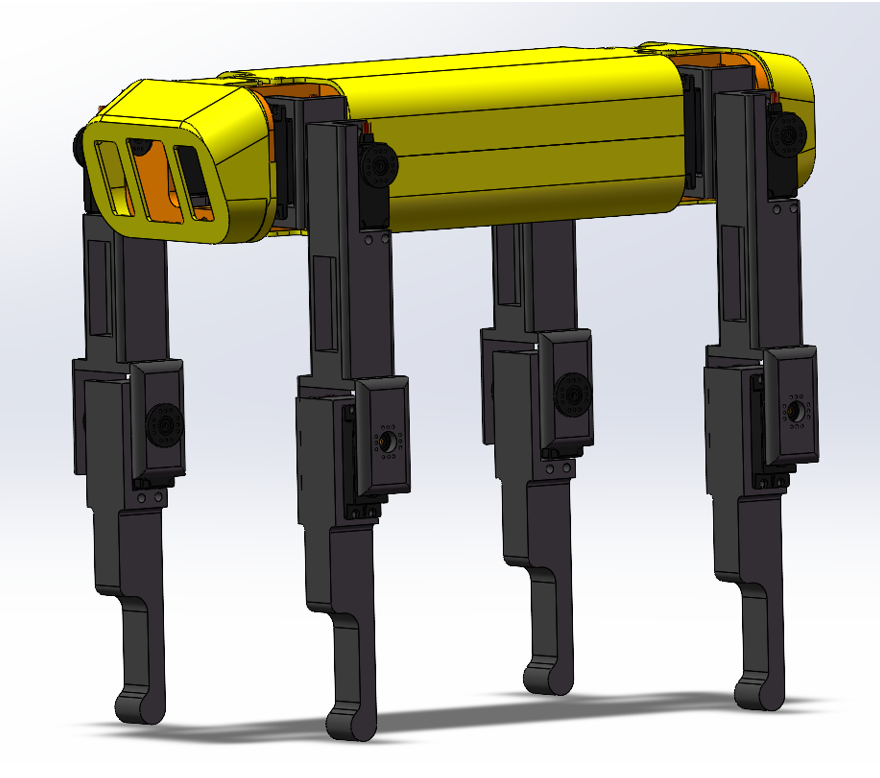
\includegraphics[height = 10cm]{fig/all.png}
	\caption{整体效果图}
	\label{all}
\end{figure}

\section{仪器核心部分设计}
\subsection{仪器检测部分和结构}
仪器监测部分需要选型传感器产品来达到一定的测量目的，这里简单介绍一下使用的产品。
\subsubsection{多模式3D距离传感器}

3D距离传感器可以用来提供二维图像和距离深度，从而可以通过一定算法来实现三维立体图像的构建，
根据原理具体可分为：
\begin{enumerate}
	\item 结构光法；
	\item 飞行时间法；
	\item 双目视差立体匹配；
\end{enumerate}
在这里介绍一种成熟产品，由卡耐基大学机器人实验室生产的MultiSense S7，如图\ref{camera}所示，其分辨率高达2Kx2K，可以通过两相机视差可以计算出物体和相机的距离；先拍摄左右两张高分辨率的图片，然后用标定内参对左右两幅图像进行了畸变校正，并对两图逐点进行像素级匹配。

\begin{figure}[htbp]
	\centering
	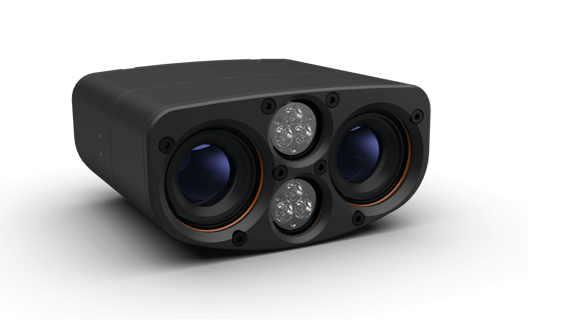
\includegraphics[height = 8cm]{fig/camera.png}
	\caption{MultiSense S7}
	\label{camera}
\end{figure}

\subsubsection{惯性导航传感器}
惯性导航仪为机构提供自身所处的位置信息以及行动过程中的运动信息，主要可分为提供平动加速度的加速度计以及旋转自由度的陀螺仪。

加速度计选用的是IIM-42351型号，是一个封装在2.5×3×0.91 mm（14针LGA）小封装中的3轴加速计。
IIM-42351具有多种功能，可在工业应用中实现简单、可靠和准确的惯性和倾斜测量，如低噪声、低功率和高达8kHz的输出数据速率。
IIM-42351的主机接口可配置为支持I3C℠ 从属、I²C从属或SPI从属模式。I3C℠ 接口支持高达12.5MHz的速度（SDR模式下的数据速率高达12.5Mbps，DDR模式下为25Mbps），I²C接口支持高至1MHz的速度，SPI接口支持高高达24MHz的速度。该设备的工作电压范围为3.6V至1.71V。

陀螺仪选用的是MPU-6050型号，MPU-6050的角速度全格感测范围为±250、±500、±1000与±2000°/sec (dps)，可准确追踪快速与慢速动作，并且，用户可程式控制的加速器全格感测范围为±2g、±4g±8g与±16g。产品传输可透过最高至400kHz的IIC或最高达20MHz的SPI（MPU-6050没有SPI）。MPU-6000可在不同电压下工作，VDD供电电压介为2.5V±5\%、3.0V±5\%或3.3V±5\%，逻辑接口VDDIO供电为1.8V± 5\%（MPU6000仅用VDD）。MPU-6000的包装尺寸4x4x0.9mm(QFN)，在业界是革命性的尺寸。其他的特征包含内建的温度感测器、包含在运作环境中仅有±1\%变动的振荡器。

\subsubsection{其他传感器}
还有其他传感器比如气压计提供高度信息，磁力计提供方位信息，从而构建整体的环境架构。

气体传感器选用的是BM1383GLV，Rohm公司推出了其新的BM1383GLV压阻式压力传感器系列，由于内置温度校正功能，该系列具有一流的压力精度和在低温和高温下的稳定测量。
采用专有MEMs技术，压阻传感元件输出与大气压力成比例的信号。该信号由使用专有算法的集成逻辑处理。这允许获得对于整个温度范围稳定的高精度压力信息。

此外，该传感器针对低功耗进行了优化，特别是针对高精度测量。内置I2C接口可确保在任何类型的移动或电池驱动应用程序中轻松访问测量结果。例如，该传感器可以通过压力变化检测高度（高度）的差异，并捕捉运动数据，这使其成为可穿戴设备、活动监视器、高度计和智能手机和平板电脑室内导航高级检测的理想解决方案。

IC封装在坚固紧凑的2.5mm x 2.5mm x 0.95mm封装中，可处理300hPA至1100hPA的宽压力范围，并提供精确的绝对值和相对压力精度。它们的电源电压为1.71至3.6V，平均电流为5uA，工作温度范围为-40℃至85℃。

而磁力计选用的是BM14270，BM14270AMUV-LB是无芯非接触式电流，使用MI传感器的磁检测传感器。它能够以非接触方式测量电流线，因此可以无损耗地测量电流。

\subsection{关键部件分析}
该结构的关键部件分为两部分，一个是中心框架的设计，另一个是腿部的设计。

\subsubsection{中心框架设计}
对于中心框架采取骨架加上外壳的设计，中心骨架由两个侧板和前后板连接，前后板分别与前后支撑架进行连接，这样形成中心框架的设计，如图\ref{center1}所示。而外壳则为上下盖板和前后盖组成，整体框架如图\ref{center2}所示。

\begin{figure}[htbp]
	\begin{minipage}{0.4\linewidth}
		\centering
		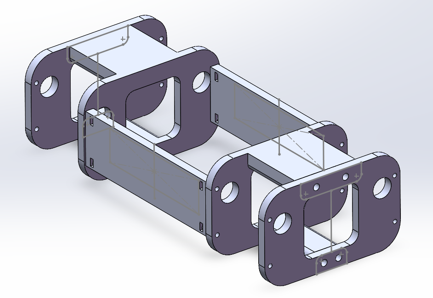
\includegraphics[height=3.5cm]{fig/center1.png}
		\caption{中心框架的骨架}
		\label{center1}
	\end{minipage}
	\hfill
	\begin{minipage}{0.6\linewidth}
		\centering
		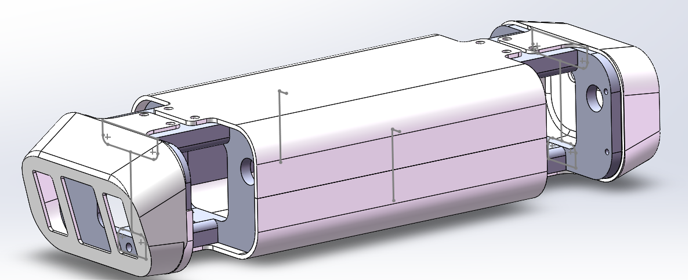
\includegraphics[height=3.5cm]{fig/center2.png}
		\caption{加上了外壳的中心框架}
		\label{center2}
	\end{minipage}
	\label{center}
\end{figure}

\subsubsection{腿部设计}
四条腿的设计相同，两侧的腿是一个镜像设计，但大致结构相同，由髋关节、大腿、小腿三部分组成，结果如图\ref{leg}所示。

\begin{figure}[htbp]
	\centering
	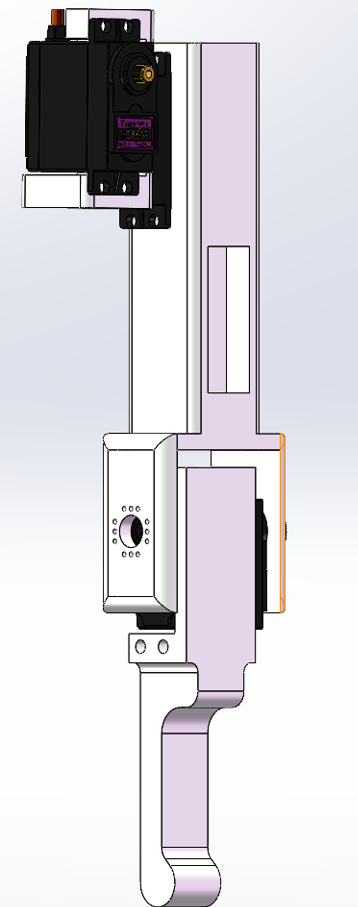
\includegraphics[height = 8cm]{fig/leg.png}
	\caption{腿部示意图}
	\label{leg}
\end{figure}

\section{主要零部件的设计计算}
\subsection{关键零件的设计}
该设计需要注意的关键设计为腿部的三部分，在尺寸、结构设计方面需要加强设计，可以通过有限元分析对原有设计进行改进。

\subsection{有限元分析}
有限元分析（FEA，Finite Element Analysis）利用数学近似的方法对真实物理系统（几何和载荷工况）进行模拟。利用简单而又相互作用的元素（即单元），就可以用有限数量的未知量去逼近无限未知量的真实系统。

\subsubsection{有限元分析的简要步骤}
这里对在Solidworks中进行有限元分析的步骤简单罗列如下：

\begin{enumerate}
	\item 建立算例进行静力学分析；
	\item 选择材料后应用；
	\item 增加夹具，添加约束；
	\item 根据具体情况施加载荷；
	\item 选定密度后划分网格；
	\item 运行算例分析结果。
\end{enumerate}

如图\ref{finite}所示即为具体分析过程时的步骤，左侧表示的是添加约束的模型，中间表示添加载荷的情况，右侧表示划分后的网格密度。
\begin{figure}[htbp]
	\centering
	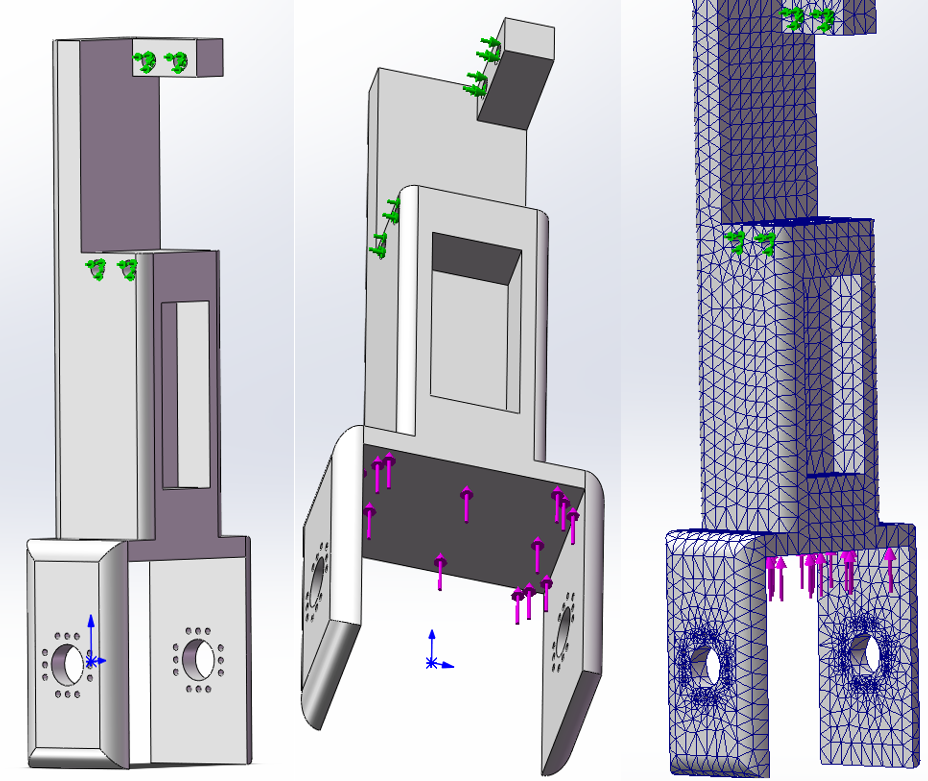
\includegraphics[height = 8cm]{fig/finite.png}
	\caption{有限元分析步骤}
	\label{finite}
\end{figure}

\subsubsection{分析不同材料的影响}

在比较各种材料时需要综合考虑材料的成本、性能、重量等影响因素，从而选取相对更好的材料，可以通过有限元分析来综合比较不同材料的表现，结合上述步骤在Solidworks中进行相应的有限元分析得到如下两种材料之间的比较，综合来看环氧树脂材料表现更好。

\begin{figure}[htbp]
	\begin{minipage}{0.45\linewidth}
		\centering
		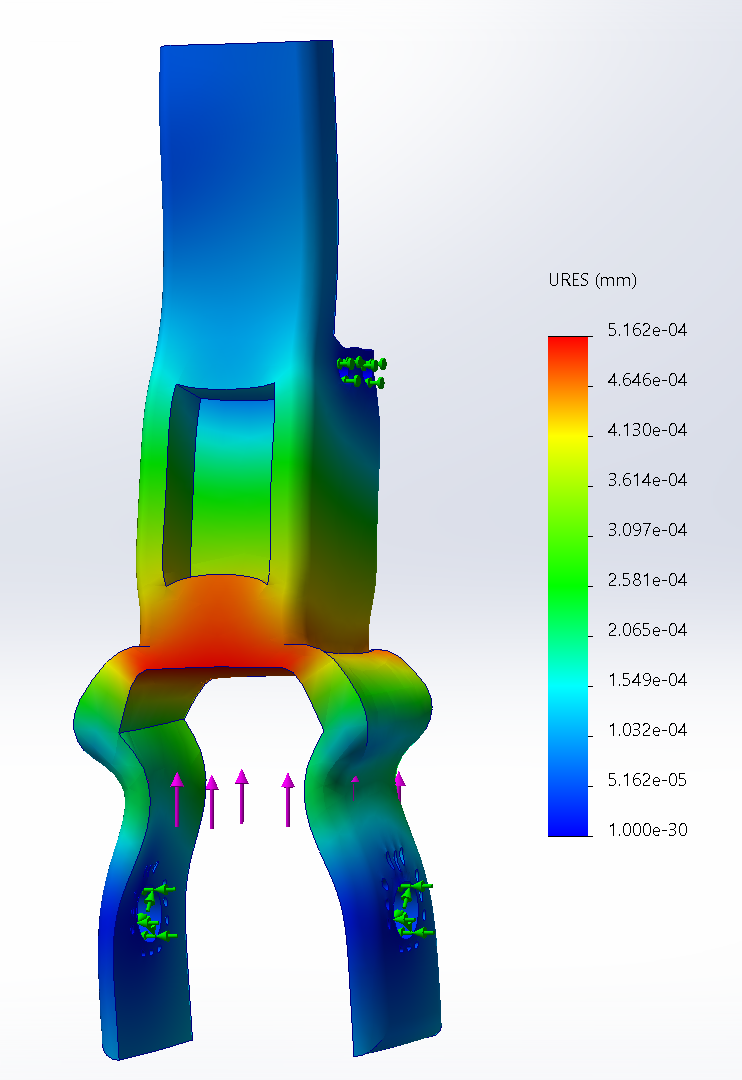
\includegraphics[height=6cm]{fig/ABS_move.png}
		\caption{ABS的位移表示}
	\end{minipage}
	\hfill
	\begin{minipage}{0.45\linewidth}
		\centering
		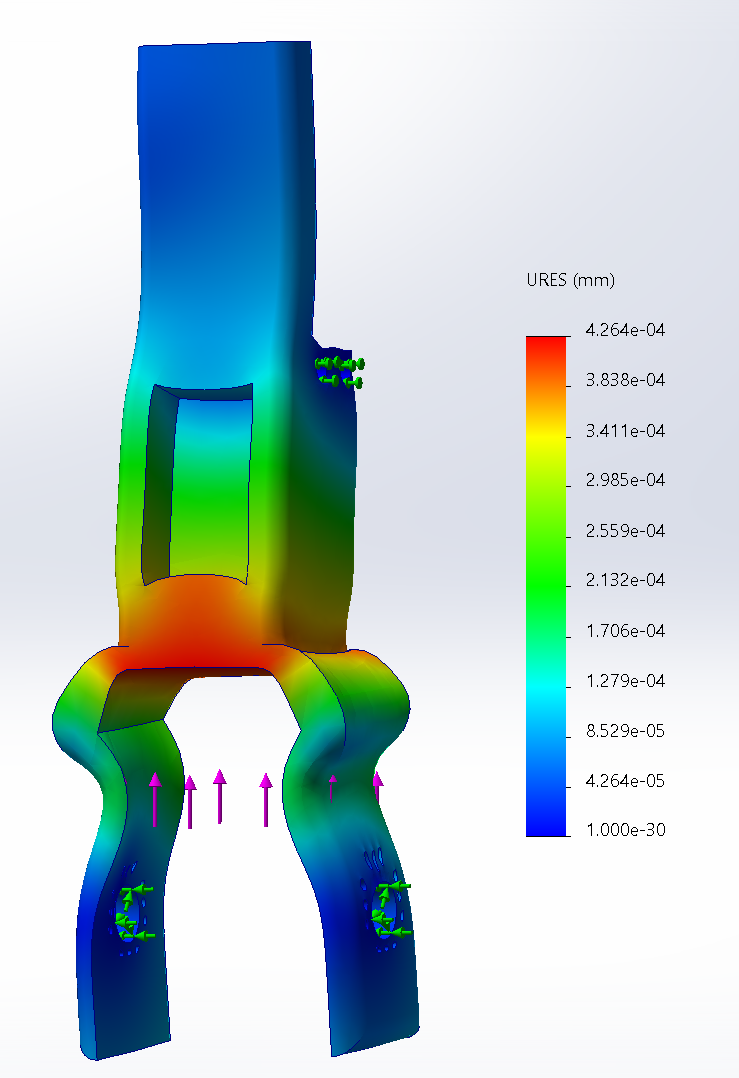
\includegraphics[height=6cm]{fig/环氧_move.png}
		\caption{环氧树脂的位移表示}
	\end{minipage}
\end{figure}

\begin{figure}[htbp]
	\begin{minipage}{0.45\linewidth}
		\centering
		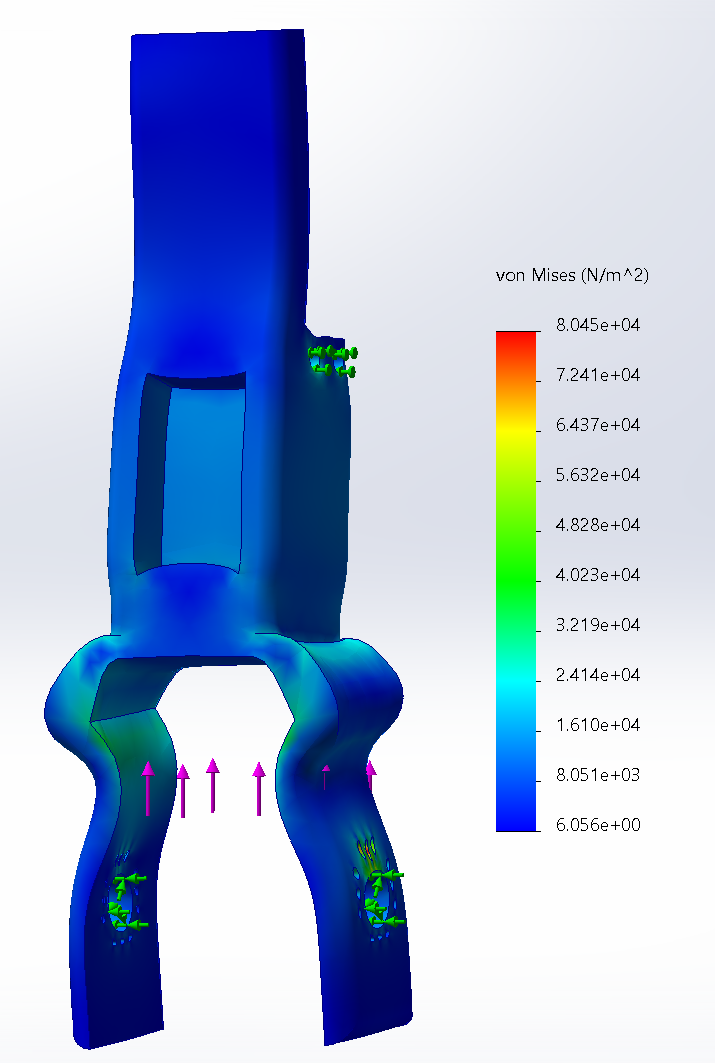
\includegraphics[height=6cm]{fig/ABS_force.png}
		\caption{ABS的应力表示}
	\end{minipage}
	\hfill
	\begin{minipage}{0.45\linewidth}
		\centering
		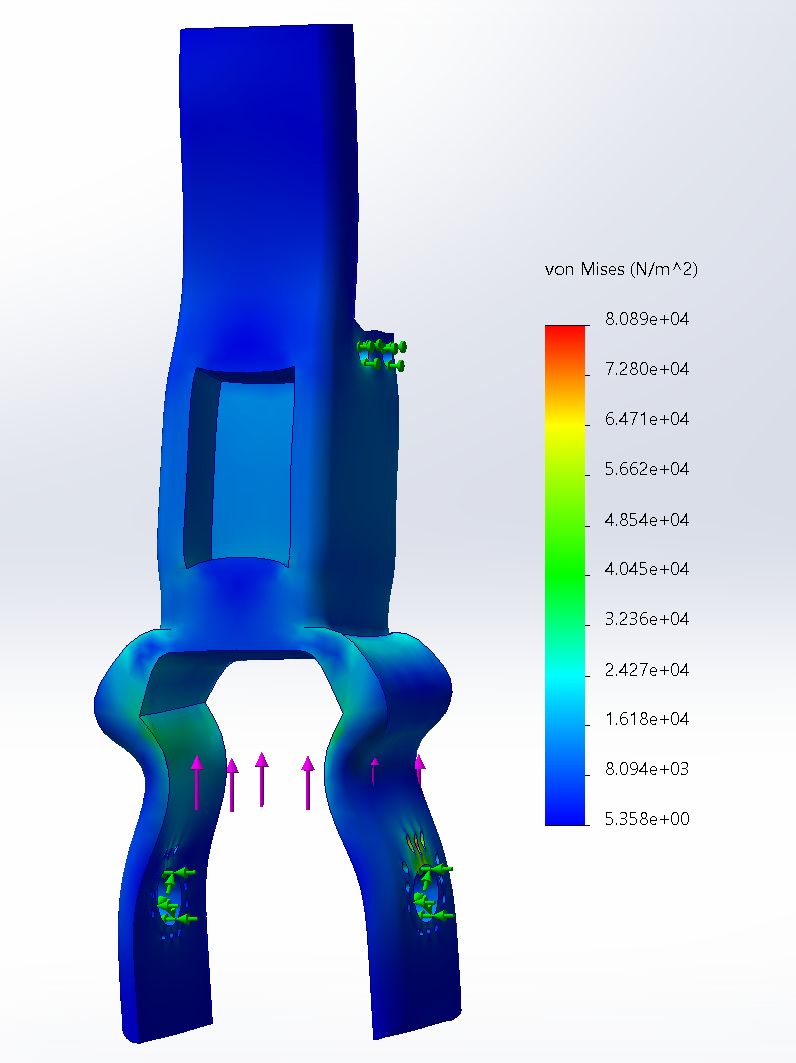
\includegraphics[height=6cm]{fig/环氧_force.png}
		\caption{环氧树脂的应力表示}
	\end{minipage}
\end{figure}


\subsubsection{对结构进行改进和优化}

对重要零件如髋关节、大腿和小腿分别进行有限元分析后进行结构方面的相关优化，对于应力和变形更大的地方进行一定程度的加强和改进，结果如下：

对于髋关节，可以看到应力和变形最大的地方在支撑的侧板和靠近侧板的螺纹孔；
\begin{figure}[htbp]
	\centering
	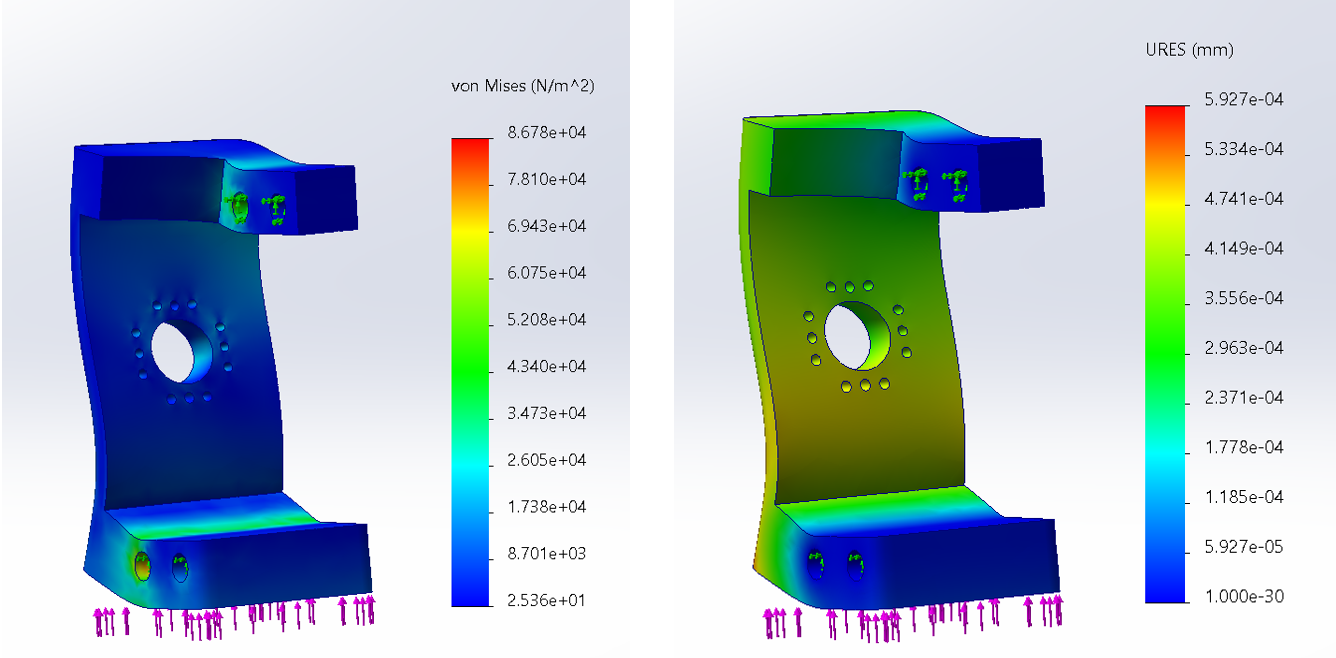
\includegraphics[width=\linewidth]{fig/leg0.png}
	\caption{髋关节的有限元分析图}
	\label{leg0}
\end{figure}

对于大腿部分，可以看到应力和变形最大的地方在下侧的支撑板和下侧两端的侧板；
\begin{figure}[htbp]
	\centering
	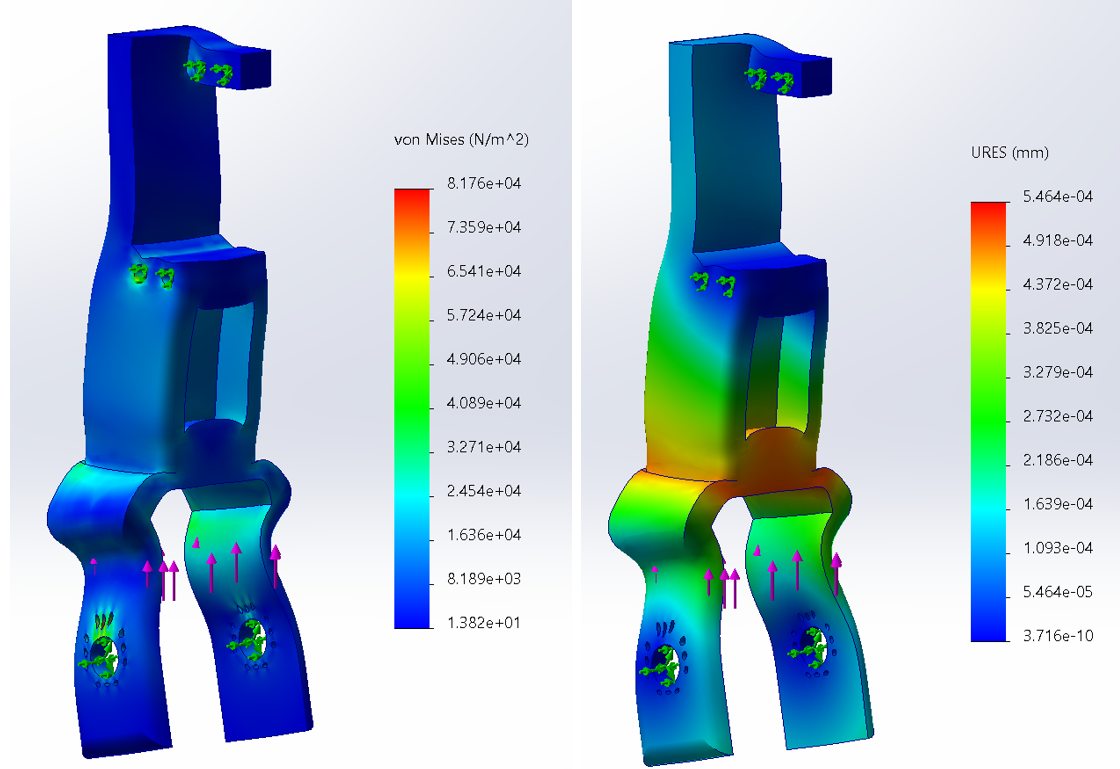
\includegraphics[height = 8cm]{fig/leg1.png}
	\caption{大腿的有限元分析图}
	\label{leg1}
\end{figure}

对于小腿部分，可以看到应力和变形最大的地方在下侧的支撑板处；
\begin{figure}[htbp]
	\centering
	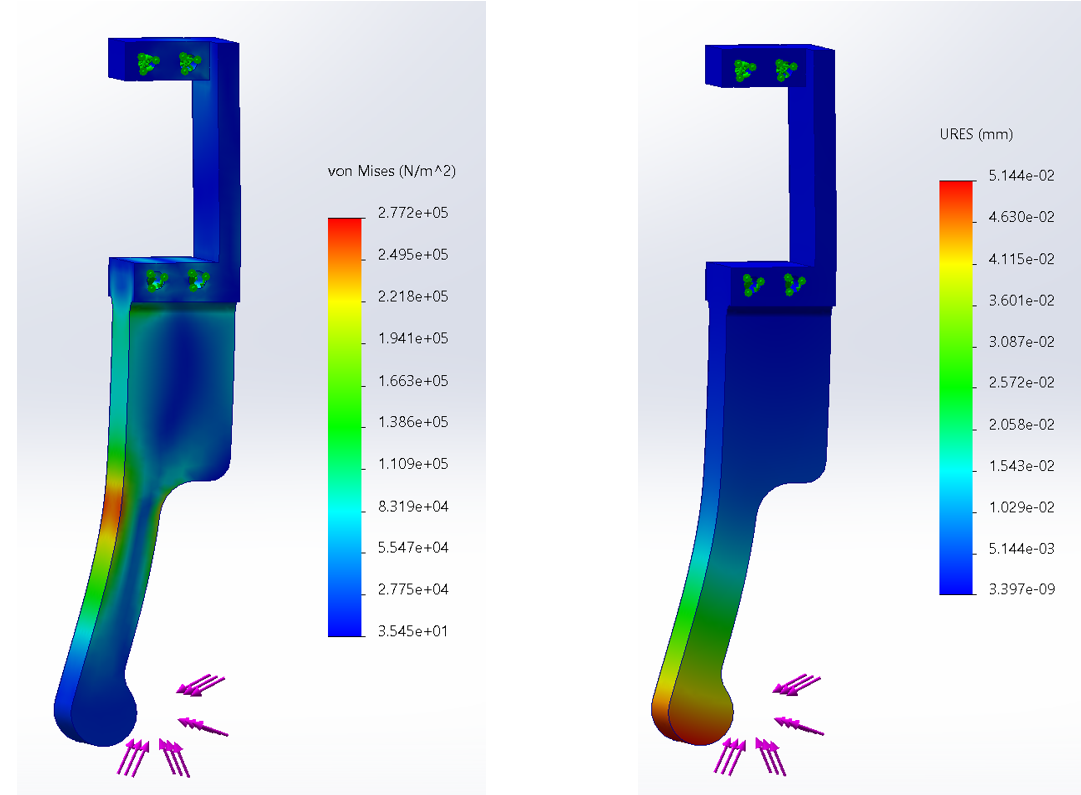
\includegraphics[height = 8cm]{fig/leg2.png}
	\caption{小腿的有限元分析图}
	\label{leg2}
\end{figure}

综上可以看到选择的材料和设计的结构可以满足需求，并可由有限元分析的结果对变形和应力更大的地方进行一定的加厚处理，并进行一定的结构优化和改进。

\subsection{整体仪器装配说明}
装配的过程分为两部分，一部分是中心骨架的组装，另一部分是腿部的组装：
\subsubsection{中心骨架的组装}
1.支撑板与前后支撑架之间进行连接，如图\ref{link1}所示；

\begin{figure}[htbp]
	\centering
	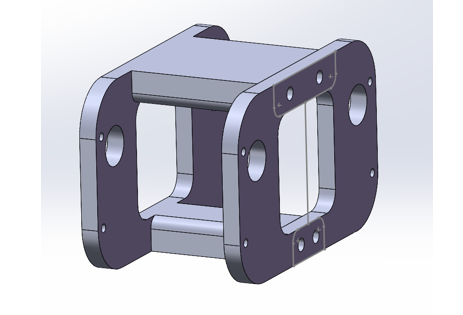
\includegraphics[height = 8cm]{fig/link1.png}
	\caption{中心骨架组装1}
	\label{link1}
\end{figure}

2.侧板与前后支撑板之间连接，如图\ref{link2}所示；

\begin{figure}[htbp]
	\centering
	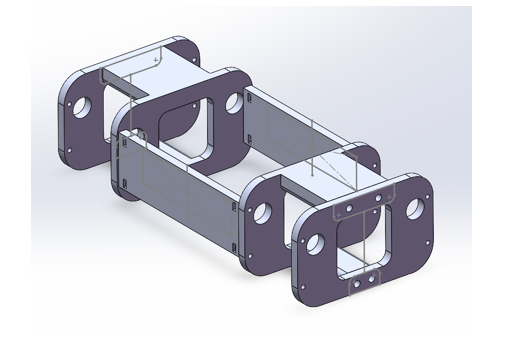
\includegraphics[height = 8cm]{fig/link2.png}
	\caption{中心骨架组装2}
	\label{link2}
\end{figure}


3.前后支撑架与上下盖板之间进行连接，如图\ref{link3}所示；

\begin{figure}[htbp]
	\centering
	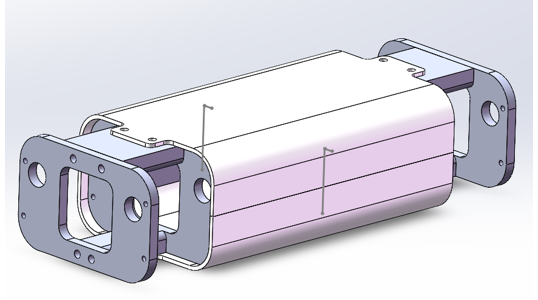
\includegraphics[height = 8cm]{fig/link3.png}
	\caption{中心骨架组装3}
	\label{link3}
\end{figure}

4.前后盖板与前后支撑架进行连接，如图\ref{link4}所示；

\begin{figure}[htbp]
	\centering
	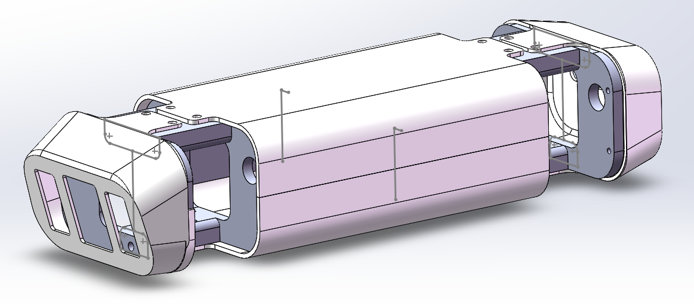
\includegraphics[width=\linewidth]{fig/link4.png}
	\caption{中心骨架组装4}
	\label{link4}
\end{figure}

\subsubsection{腿部的组装}
1.将电机与髋关节、大腿和小腿分别进行组装，如图\ref{link5}所示；

2.将髋关节与大腿连接后再与小腿连接，如图\ref{link6}所示；
\begin{figure}[htbp]
	\begin{minipage}{0.45\linewidth}
		\centering
		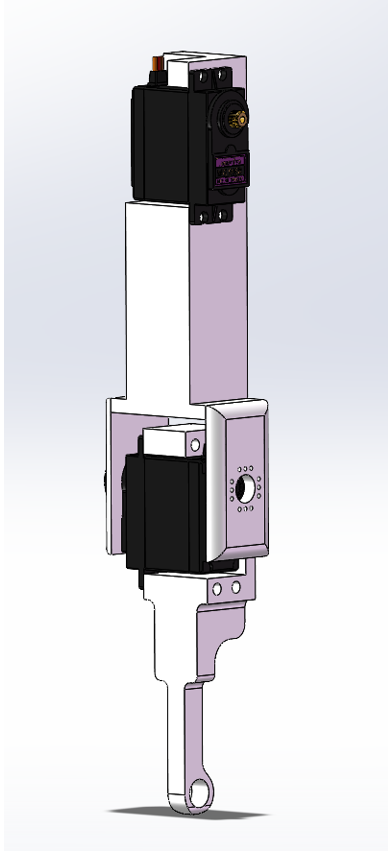
\includegraphics[height=6cm]{fig/link5.png}
		\caption{腿部装配1}
		\label{link5}
	\end{minipage}
	\hfill
	\begin{minipage}{0.45\linewidth}
		\centering
		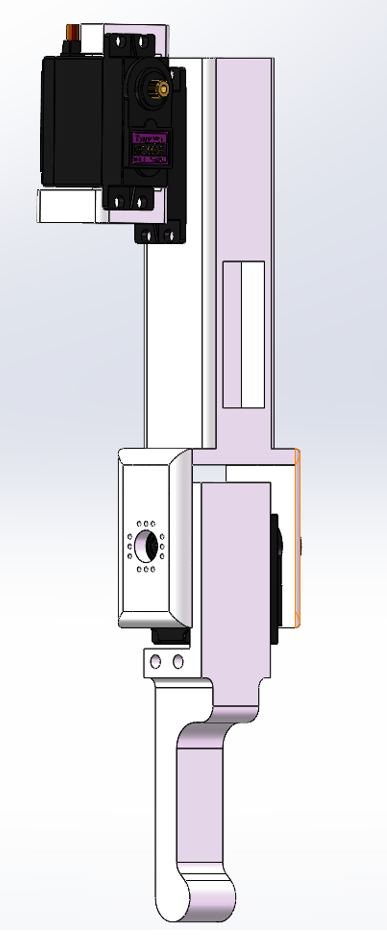
\includegraphics[height=6cm]{fig/link6.png}
		\caption{腿部装配2}
		\label{link6}
	\end{minipage}
\end{figure}

\section{主要零件制造工艺设计}
\subsection{零件工艺性分析}
工艺分析的目的，一是审查零件的结构形状及尺寸精度的技术要求是否合理，是否便于加工和装配；二是通过工艺分析，对零件的工艺要求有进一步的了解,以便制订出合理的工艺规程。根据具体的技术要求可以制定相应的加工方法，在工艺卡片中给予更详细的描述。

\subsection{加工设备选择}

由于材料为环氧树脂，并且使用分体式结构，对于尺寸和材料的要求都可以被3D打印满足，所以材料成型可以使用3D打印机，其余的孔和毛刺的加工使用钻床来铰孔，去毛刺使用砂轮机或者手工打磨即可满足要求。

\section{运动学分析与建模}
\subsection{腿部运动模型建立}
在进行运动学分析之前需要对需要研究的三自由的腿部物理模型进行数学模型的抽象，从而方便实际分析。可以把腿部抽象为如图的连杆机构，每两个连杆之间由一个旋转自由度进行联接。

\subsection{正运动学分析}
正运动学是通过三个舵机各自的旋转角度来确定足部末端的三维位置点的过程。
按照图      所示建立腿部模型并选定坐标系，则可进行相应的坐标分析如下：
在xyz坐标系下，设定A为原点，则B坐标为 $(h_0cos\alpha, h_0sin\alpha, 0)$

在x'y'z'坐标系下，以B'为原点，则D'坐标为 $(0, -h_1sin\beta-h_2sin(\beta+\gamma), -h1cos\beta-h_2cos(\beta+\gamma))$

由x'y'z'坐标系到xyz坐标系的变换公式为

\begin{equation}
	\left(
		\begin{array}{c}
			x \\
			y \\
			z
		\end{array}
	\right)
	=
	\left(
		\begin{array}{ccc}
			cos\alpha & -sin\alpha & 0 \\
			sin\alpha & cos\alpha & 0 \\
			0 & 0 & 1
		\end{array}
		\begin{array}{c}
			x' \\
			y' \\
			z' 	
		\end{array}
		+
		\begin{array}{c}
			x^B \\
			y^B \\
			z^B 	
		\end{array}
	\right)
\end{equation}

套用坐标变换公式即可得到D点在xyz坐标系里的坐标为：

\begin{equation}
	\left(
		\begin{array}{l}
			x_D \\
			y_D \\
			z_D
		\end{array}
	\right)
	=
	\left(
		\begin{array}{l}
			h_0cos^2\alpha+h_1sin\alpha sin\beta+h_2sin(\beta+\gamma)+h_0cos\alpha \\
			h_0sin\alpha cos\alpha - h_1cos\alpha sin\beta - h_2cos\alpha sin(\beta+\gamma)+h_1sin\alpha \\
			-h_1cos\beta - h_2cos(\beta+\gamma)
		\end{array}
	\right)
\end{equation}

至此即完成了正运动学的分析，当已知三个关节的旋转角度时即可计算D点在绝对坐标系下的坐标。

\subsection{逆运动学分析}
逆运动学是通过确定所需要的三维位置点坐标后，反向对三个舵机的旋转角度进行确定的过程，在实际使用过程中更实用。

在当前的腿部模型下，在xyz坐标系的xy平面投影内，BCD三个点的投影必然共线，为了使得D点落到指定位置点，则需要使得BCD的投影直线经过设定点的投影点坐标

有一定几何关系可以算得

\begin{equation}
	\alpha = \theta_1 + \theta_2 = arctan \frac{y_D}{x_D} + arccos \frac{h_0}{\sqrt[2]{x_D^2 + y_D^2}}
\end{equation}

与正运动学分析时的变换相反，由xyz坐标系到x'y'z'坐标系的变换公式为

\begin{equation}
	\left(
		\begin{array}{c}
			x' \\
			y' \\
			z'
		\end{array}
	\right)
	=
	\left(
		\begin{array}{ccc}
			cos\alpha & sin\alpha & 0 \\
			-sin\alpha & cos\alpha & 0 \\
			0 & 0 & 1
		\end{array}
		\begin{array}{c}
			x-x_B \\
			y-y_B \\
			z-z_B 	
		\end{array}
	\right)
\end{equation}

则在x'y'z'坐标系内，由三角关系可得到如下方程组：

\begin{equation}
	\left\{
	\begin{array}{l}
		\gamma = 180^\circ - \delta \\
		\delta = arccos \frac{h_1^2+(h_2)^2-((y')_D^2+(z')_D^2)}{2h_1 h_2} \\
		\omega = arccos \frac{h_1^2+(y')_D^2+(z')_D^2-h_2^2}{2h_1 sqrt{(y')_D^2+(z')_D^2}} \\
		\beta + \omega = arctan \frac{(z')_D^2}{(y')_D}
	\end{array}
	\right.
\end{equation}

可以解得到$\beta$和$\gamma$的解析解。

综上，给定D点坐标后，三个角度如下：
\begin{equation}
	\left\{
	\begin{array}{l}
		\alpha = arctan \frac{y_D}{x_D} + arccos \frac{h_0}{sqrt{x_D^2+y_D^2}} \\
		\beta = arctan \frac{z}{ycos \alpha - xsin\alpha} - arccos \frac{(y\cos\alpha-x\sin\alpha)^2+h_1^2-h_2^2+z^2}{2h_1\sqrt{(y\cos\alpha-x\sin\alpha)^2+z^2}} \\
		\gamma = \arccos \frac{(y\cos\alpha-x\sin\alpha)^2-h^2_1-h_2^2+z^2}{2h_1h_2}
		
	\end{array}
	\right.
\end{equation}


\subsection{运动空间分析}
在实际使用过程中还需要注意运动空间的分析，因为受限于腿部自身尺寸和旋转角度，模型计算的公式对于一些情况不再适用，所以需要对三维空间点的坐标进行限制。下面就分析了工作空间的
限制，并遍历了三维空间的很多离散点来直观显示工作空间。以下为源代码内容：

\lstset{numbers=left, %设置行号位置
        numberstyle=\tiny, %设置行号大小
        keywordstyle=\color{blue}, %设置关键字颜色
        commentstyle=\color[cmyk]{1,0,1,0}, %设置注释颜色
        frame=single, %设置边框格式
        escapeinside=``, %逃逸字符(1左面的键)，用于显示中文
		breaklines, %自动折行
        extendedchars=false, %解决代码跨页时，章节标题，页眉等汉字不显示的问题
        xleftmargin=2em,xrightmargin=2em, aboveskip=1em, %设置边距
        tabsize=4, %设置tab空格数
        showspaces=false %不显示空格
       }

\begin{lstlisting}[language=Matlab]
	% Define some variables
	H0 = 1;
	H1 = 1;
	H2 = 1;
	
	% Loop to find out the workspace
	for x=0:0.02:H0
		for y=0:0.02:H1+H2
			for z=0:0.02:H1+H2
				%Check the feasibility
				a = rad2deg(atan(y/x)+acos(H0/sqrt(x^2+y^2)));
				yd = y*cos(a)-x*sin(a);
				zd = z;
	
				if( (x^2+y^2)<H0^2 || sqrt(yd^2+zd^2)>(H1+H2))
					fprintf("%.3g %.3g %.3g is out of Reach!\n",x, y, z);
					continue;
				end
				scatter3(x,y,z);
				hold on;
			end
		end
	end
\end{lstlisting}
	
\begin{figure}[htbp]
	\centering
	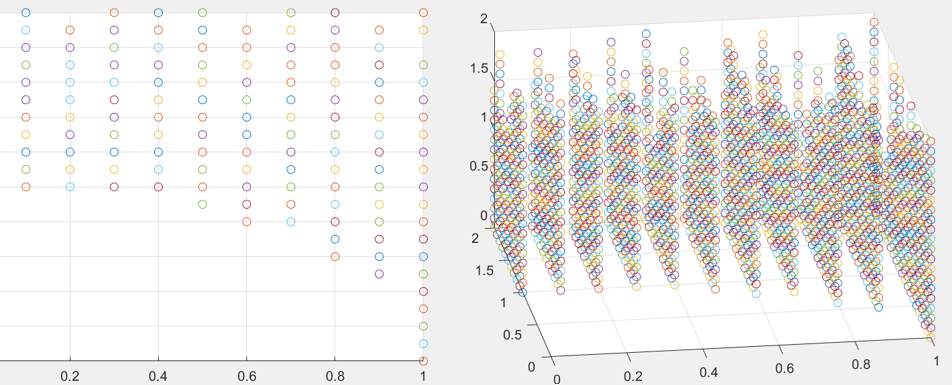
\includegraphics[height = 6cm]{fig/workspace.png}
	\caption{单位三维空间的工作范围}
	\label{workspace}
\end{figure}

运行代码即可得到在单位三维空间里的运动空间的覆盖范围，结果如图\ref{workspace}，从结果中可以观察到：在当前三个长度设定条件下，由于受限于连杆之间连接的自由度，第一根杆长覆盖的圆形区域是无法覆盖的，还有远端的一些点由于距离过远所以也无法覆盖。


\subsection{运动学公式计算}
由之前的分析可以把计算的公式和定义域转换为科学计算的代码，本文在Matlab里开展了此项工作，源代码如下：

\lstset{numbers=left, %设置行号位置
        numberstyle=\tiny, %设置行号大小
        keywordstyle=\color{blue}, %设置关键字颜色
        commentstyle=\color[cmyk]{1,0,1,0}, %设置注释颜色
        frame=single, %设置边框格式
        escapeinside=``, %逃逸字符(1左面的键)，用于显示中文
		breaklines, %自动折行
        extendedchars=false, %解决代码跨页时，章节标题，页眉等汉字不显示的问题
        xleftmargin=2em,xrightmargin=2em, aboveskip=1em, %设置边距
        tabsize=4, %设置tab空格数
        showspaces=false %不显示空格
       }

\begin{lstlisting}[language=Matlab]
%Define the constant variables
H0=100;
H1=100;
H2=100;

%Calculate
while(1)
    % input the axises of D
    x = input("please input the x: \n");
    y = input("please input the y:\n");
    z = input("please input the z:\n");
    
    % Calculate the angles for D
    a = rad2deg(atan(y/x)+acos(H0/sqrt(x^2+y^2)));
    b = rad2deg(atan(z/(y*cos(a)-x*sin(a)))-acos(((y*cos(a)-x*sin(a))^2+H1^2-H2^2+z^2)/...
        (2*H1*sqrt((y*cos(a)-x*sin(a))^2+z^2))));
    c = rad2deg(acos(((y*cos(a)-x*sin(a))^2-H1^2-H2^2+z^2)/(2*H1*H2)));
    
    %Check the feasibility
    if( (x^2+y^2)<H0^2 )
        fprintf("Error! Out of Reach!\n\n");
        continue;
    end

    yd = y*cos(a)-x*sin(a);
    zd = z;
    if( sqrt(yd^2+zd^2)>(H1+H2))
        fprintf("Error! Out of Reach!\n\n");
        continue;
    end
    
    % Print the results
    fprintf("the alpha is %.2g \n",a);
    fprintf("the beta is %.2g \n",b);
    fprintf("the gamma is %.2g \n\n",c);
end

\end{lstlisting}


\begin{figure}[htbp]
	\centering
	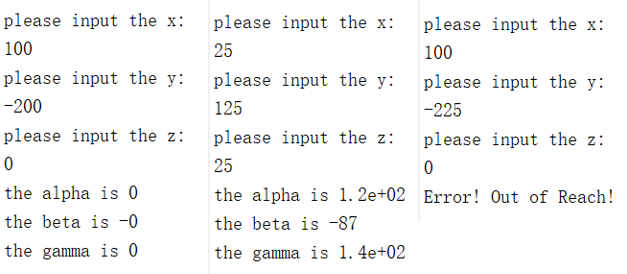
\includegraphics[height = 5cm]{fig/result.png}
	\caption{程序测试输出结果}
	\label{result}
\end{figure}

从图\ref{result}可以看到，对于初始状态和一般状态，该公式都可以正确输出结果，并且对于超出了工作空间的情况也可输出报错提示，说明该工作符合预期。

\subsection{运动学建模}
在建立了物理模型，并分析了运动学原理之后，便可以对运动学进行模型，利用Matlab中的Simulink模块里的多体物理仿真部分，可以对该机器狗进行运动学仿真建模。

Simulink是一个模块图环境，用于多域仿真以及基于模型的设计。它支持系统设计、仿真、自动代码生成以及嵌入式系统的连续测试和验证。Simulink提供图形编辑器、可自定义的模块库以及求解器，能够进行动态系统建模和仿真。

在导入机器狗的物理模型后，添加关节处的旋转自由度限制，并对足部和底板之间的物理交互进行规定，在对各关节的运动波形做出规定之后即可使机器狗进行运动。根据仿生学，机器狗具有诸多的步态都可以进行相应的波形规划来实现运动，我们将足式动物的运动模式定义为“步态”，指的就是足式动物各腿之间的固定相位关系。受限于篇幅，这里仅对各种步态进行描述，而并没有对各个步态的波形模式进行模拟仿真。以下列举三种常见步态的模式和特点：
\begin{enumerate}
	\item crawl步态：慢速行走状态，在任意时刻都有三条腿处于支撑相，一条腿处于摆动相；
	\item trot步态：小跑状态，在任意时刻处于对角位置的两对腿分别处于支撑相和摆动相；
	\item pace步态：溜蹄步态：相同侧的两条腿为相同状态，两侧分别处于支撑相和摆动相；
\end{enumerate}
对于不同步态还可以调整运动的占空比和步态周期来实现不同的运动效果。


\begin{figure}[htbp]
	\centering
	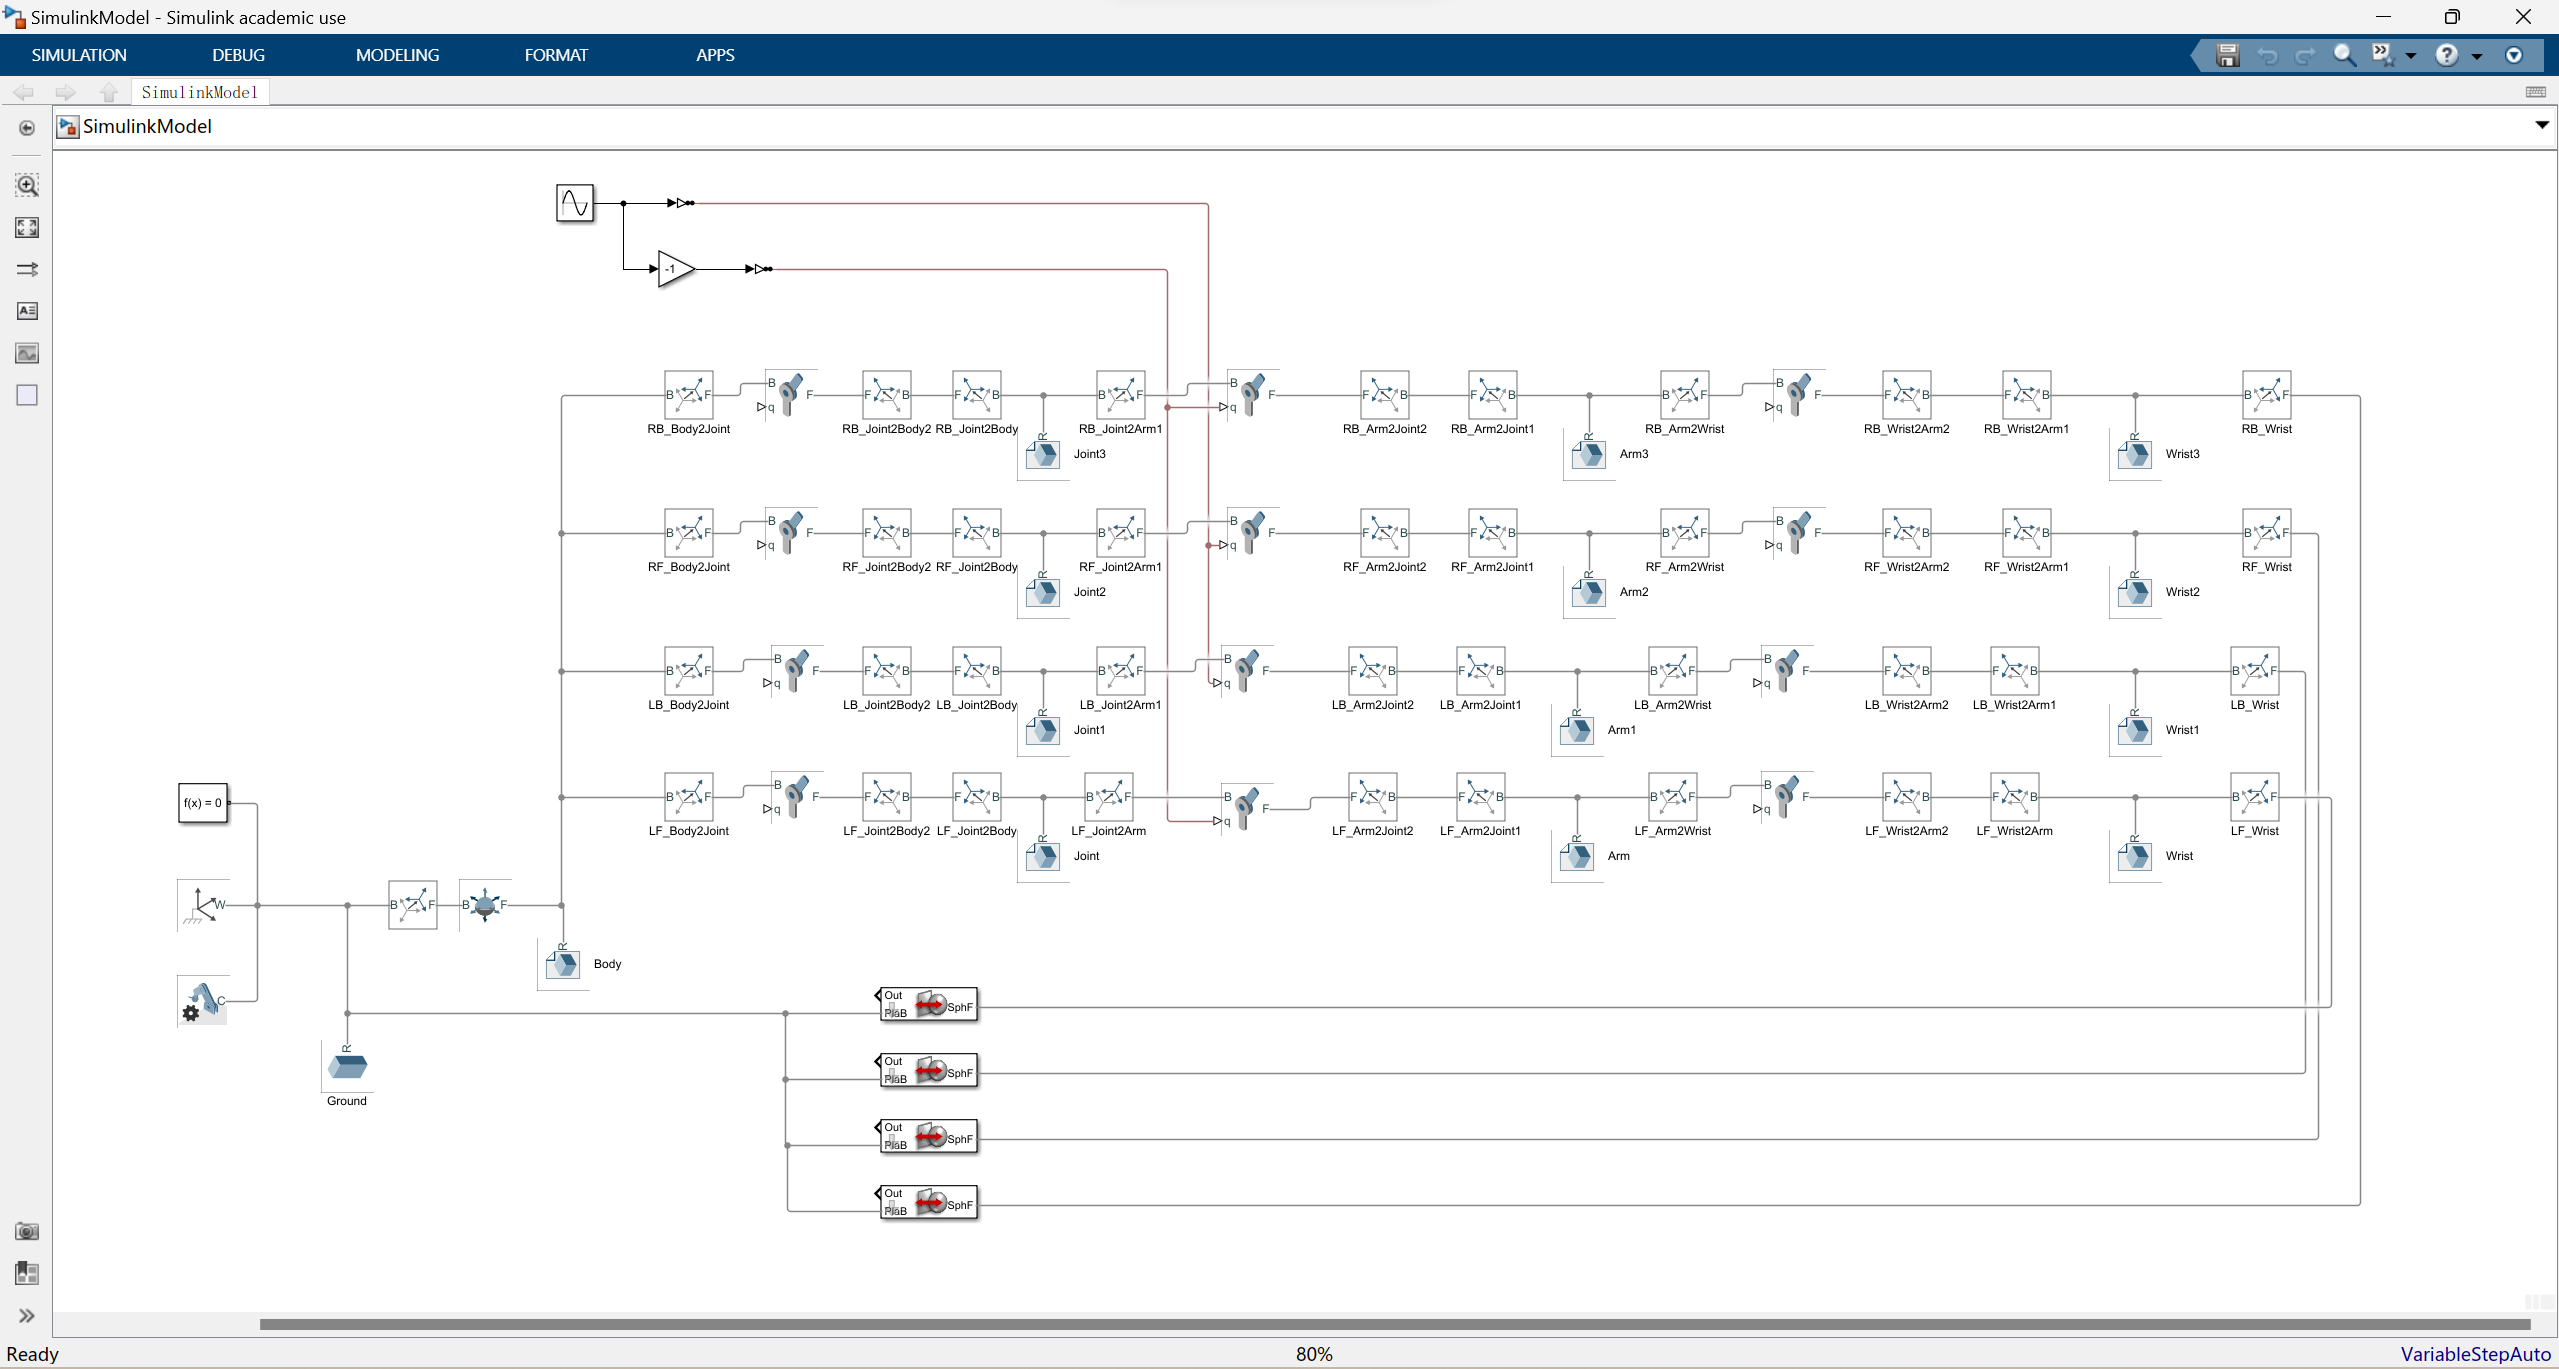
\includegraphics[width=\linewidth]{fig/simulink.png}
	\caption{Simulink里的模块仿真图}
	\label{simulink}
\end{figure}

如图\ref{simulink}为在Simulink模块里的多体仿真模块示意图。该模型导入了机器狗的物理模型，并分别对四条腿都添加了相应的关节约束关系；下方为四条腿末端的力反馈模块，用来提供地面与足部之间的力反馈；上方的波形发生器为四条腿的运动进行了简单的运动规划，从而可以实现在Simulink里的简单运动，若想要实现更复杂的步态规划，则可以在波形发生器的地方控制输出的波形，并将其添加到其他关节处，从而实现更复杂的步态行进。

\begin{figure}[htbp]
	\centering
	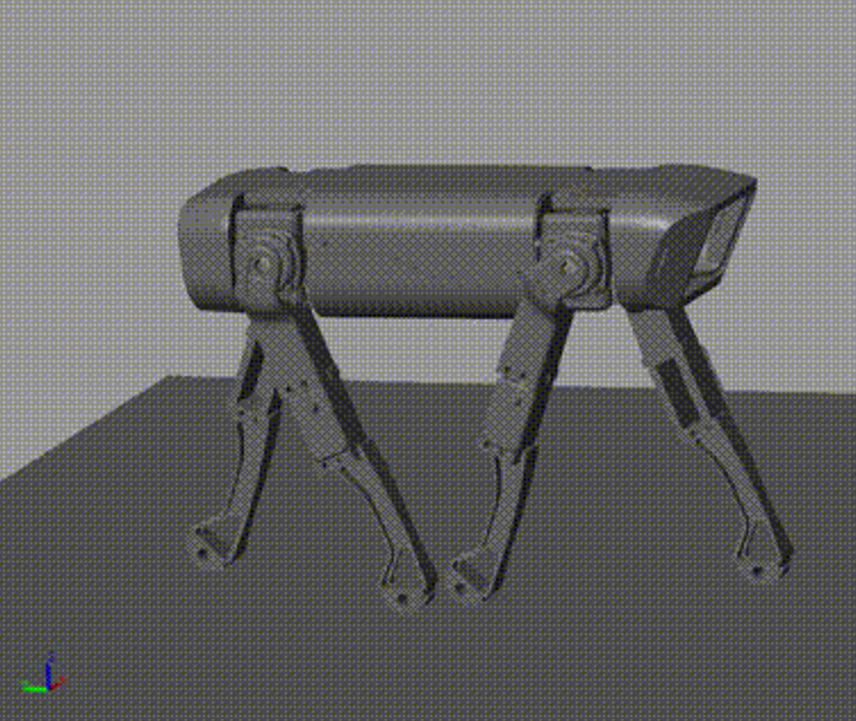
\includegraphics[height = 8cm]{fig/walk.png}
	\caption{Simulink仿真结果}
	\label{walk}
\end{figure}

仿真的结果输出如图\ref{walk}所示，在添加了力学仿真和简单运动波形后，机器狗可以实现在平地上的简单行走，效果较好。

\section{设计小结}
\subsection{设计特点}
该设计对机器狗设计过程的诸多方面进行了总结和尝试，在进行了相关背景调研之后，从物理建模开始设计各部件的形态和配合关系，并对电机等其他器件进行选型。在设计过程中还通过有限元分析来确定设计的合理性，并在模型设计和材料选择的方面进行一定指导。在建模完成后还对各个部件的工艺进行设计，从而为具体实践提供帮助。物理建模完成后还要进行运动学的建模去明确各关节的运动关系，分别进行正逆运动学分析得到坐标和角度之间的对应关系，同时要对运动空间分析，得到腿部末端可以到达的空间区域。本文还将设计的物理模型导入到Simulink当中进行了运动仿真，可以在模型中对四条腿的运动进行规划，从而实现不同的运动效果。


\subsection{问题和发展}
该四足机器狗在一些方面还有改进的空间，还可能存在更深层次的问题需要实际组建后才能够发现。

比如可以对机器狗的运动方式进行结构改进，结合足式机器人和轮式机器人的优点，构造轮足复合型的机器狗，在复杂地形时采用足式运动，增强运动能力和运动能力，对于转弯等场景具有更强的灵活性；而在平整且空旷的地面环境可以采用
轮式运动，从而可以快速运动增强运动效率；具体实现可在腿部膝关节处增加万向轮，并使用电机驱动，在需要变换运动方式的时候，腿部可以进行折叠或者伸展来实现切换运动方式的功能，使该机器狗拥有更好的环境适应力。

而如果为了精确控制关节的位置，在原有基础上还可以在腿部关节处额外增加角度传感器来监测每次运动的角度是否到位，并结合姿态控制来对整个机构的运动实现更高的精度控制，具体实现可以在关节处的结构更换为轴系，然后和电机搭配码盘来实现角度的控制功能。

\newpage
\renewcommand\bibname{参考文献}
\renewcommand\refname{参考文献}
\bibliography{bib}
\bibliographystyle{plain}
\nocite{*}                  %show all the bibliography no matter what
%xelatex/bibtex/xelatex*2


\end{document}
